\section*{\LARGE Supplementary Material}

\vspace*{20pt}
\section*{Table of Contents}
\vspace*{-5pt}
\startcontents[sections]
\printcontents[sections]{l}{1}{\setcounter{tocdepth}{2}}

\newpage

\section{Breakdown of Story Attribution}
\label{appx:breakdown}

\subsection{Call for Anecdotes}

Below is the call for anecdotes we put out into our various networks and public social media sites. In addition to posting to our various networks, we reached out to some researchers directly if we believed there was a chance that they had a story that would fit this collection or if they had previously shared such a story with us, e.g., over drinks at a conference:

\begin{mdframed}[
    backgroundcolor=black!2,
    linecolor=black!35,
    linewidth=0.8pt,
    roundcorner=4pt,
    innertopmargin=10pt,
    innerbottommargin=10pt,
    innerleftmargin=12pt,
    innerrightmargin=12pt,
    skipabove=\baselineskip,
    skipbelow=\baselineskip
]
\small

Dear colleagues,

\textbf{TL;DR:} Please submit (to aifindsaway@gmail.com) any stories you know of where AI acted in a way that surprised its creators, especially if it could be seen as unsafe (e.g. hacking a reward function, finding a loophole in an environment or experimental design, goal misgeneralization, etc.).

As AI researchers, we know that AI is creative and constantly surprises us, often outwitting our experimental designs and forcing us to iterate to close loopholes on things like reward functions and environment configurations. To anthropomorphize, it can seem mischievous or clever at times. These stories are important as society grapples with the question of AI Safety and Existential Risk, as they teach us how the unexpected is routine, and how we often fail to anticipate ways in which AI will escape our attempts to contain it. Such stories thus inform scientists, the general public, and regulators. However, these important anecdotes are usually passed around orally, meaning we do not know to what extent they are true, and it is hard for scientists and regulators to include them in official documents. To remedy these issues, we aim to record the true accounts of as many anecdotes as possible regarding AI (of any type, including RL, ML, etc.) surprising its creators and users.

This effort (by Aaron Dharna, Cong Lu, Joel Lehman, Victoria Krakovna, and Jeff Clune) is a follow-up to our 2018 paper The Surprising Creativity of Digital Evolution (TSCDE). That paper is a crowdsourced collection of anecdotes from the artificial life and evolutionary computation communities about how their algorithms creatively subverted expectations. That paper made an important contribution to ongoing discussions of AI Safety, but was limited because its scope was confined to one narrow area of AI (evolutionary methods). Our new paper expands the scope to all areas of AI, especially the most powerful methods (deep learning, including deep reinforcement learning).

This expansion of previous work is driven in part by the response of the AI Safety community to TSCDE, which has become a valuable resource for them in publications [1, 2, 3] and in teaching future leaders in AI safety by being included in AI safety course syllabi (e.g. UC Berkeley's Safety and Control for Artificial General Intelligence course).

Please send us any accounts you think we should include. If we add it to the paper, the scientists involved will be appropriately cited and/or mentioned to give them credit. Unfortunately, we ran into many challenges throughout the process with TSCDE with submitters as co-authors, so this time we are instead recognizing contributors by name and with all appropriate citations in the paper. If you know of an account but did not perform the experiment yourself, please tell us what you know, including who we might contact for a firsthand account.

We hope you can help create an account of these fascinating and sometimes ominous anecdotes so we can inform AI safety discussions, either by submitting and/or spreading the word of this Call for Anecdotes.

More details below.

Thanks,

Aaron, Cong, Joel, Victoria, and Jeff

\medskip

Please send us a quick summary of your anecdote. We can then let you know if we will include it in the paper, at which point we may ask for more details.

An example anecdote is available here, which can serve as a rough guide to the length, level of detail, and surprise factor we are looking for. Please copy the document and use it as a template for submissions. We will curate and edit these into a full publication. Before the camera-ready publication is released, we will provide you with the opportunity to read the paper and make sure you are happy with your contribution.

Please forward this email to whomever you think might have an interesting anecdote to share. We look forward to your exciting, amusing, worrisome, and/or insightful contributions!

\medskip
\textbf{References}

[1] Jess Whittlestone, Kai Arulkumaran, and Matthew Crosby. ``The Societal Implications of Deep Reinforcement Learning''. In: Journal of Artificial Intelligence Research 70 (Mar. 2021). issn: 1076-9757. doi: 10.1613/jair.1.12360. url: http://dx.doi.org/10.1613/jair.1.12360.

[2] Tom Everitt, Gary Lea, and Marcus Hutter. ``AGI Safety Literature Review''. In: IJCAI'18. Stockholm, Sweden: AAAI Press, 2018, pp. 5441-5449. isbn: 9780999241127

[3] Robert Geirhos et al. ``Shortcut learning in deep neural networks''. In: Nature Machine Intelligence 2.11 (Nov. 2020), pp. 665-673. issn: 2522-5839. doi:10.1038/s42256-020-00257-z

\end{mdframed}

\newpage

\subsection{List of Anecdotes}

10 of the anecdotes come from the public record. The remaining 16 are new to this collection.

\begin{itemize}
    \item \Cref{sec:alphago}: David Silver's section comes from his interview with Lex Fridman~\citep{silverInterviewFridman2020}; Marc Lanctot's is new; therefore, we count this as both a new addition and an item pulled from the public record.
    \item \Cref{sec:libratus}: comes from Noam Brown's interview with Kanjun Qiu at Imbue~\citep{KanjunAndNoam}
    \item \Cref{sec:diplomacy}: new
    \item \Cref{sec:opponentshaping}: new
    \item \Cref{sec:boatracing}: comes from the OpenAI blog post~\citep{OpenAI_Faulty_2016}
    \item \Cref{sec:smacshield}: new
    \item \Cref{sec:claw}: comes from the OpenAI blog post~\citep{OpenAI_Learning_2017}
    \item \Cref{sec:paired}: details of the reward hacking/collusion between agents are new to this work, but the experimental setup is described in \citet{dennis2020emergent}
    \item \Cref{sec:cyclegan}: new
    \item \Cref{sec:pokemon}: new
    \item \Cref{sec:hideseek}: comes from the OpenAI blog post~\citep{baker2019emergent} and Jeff Clune
    \item \Cref{sec:ppga}: new
    \item \Cref{sec:worldmodels}: comes from David Ha's blog post version of the published paper about World Models~\citep{ha2018world}
    \item \Cref{sec:smachandoff}: new
    \item \Cref{sec:radio}: comes from \citet{BirdRadio}
    \item \Cref{sec:gptcaptcha}: comes from OpenAI's technical report on GPT-4~\citep{openai2024gpt4, arcUpdateGPT4}
    \item \Cref{sec:vpt}: new
    \item \Cref{sec:motif}: new
    \item \Cref{sec:acescodegen}: new
    \item \Cref{sec:rainbow}: new
    \item \Cref{sec:wedding}: comes from a blog post and responding comment from Paul Christiano~\citep{christianoweddingparties}
    \item \Cref{sec:claudeneedle}: comes from the Twitter post~\citep{claude3tweet}
    \item \Cref{sec:fusion}: comes from Riedmiller's interview on the TalkRL podcast~\citep{TalkRL_Riedmiller_2023}
    \item \Cref{sec:funsearch}: some details are described in \citet{RomeraParedes2023}, but new details were provided by Alex Novikov as well, so this counts as new
    \item \Cref{sec:aiscientist}: some details were described in \citet{sakana2024aiscientist_blog}, but Cong Lu provided new details too, so this counts as new
    \item \Cref{sec:quantum}: new
\end{itemize}


\clearpage

% \section{Figures for FunSearch}

% In the Nature paper about FunSearch (\Cref{sec:funsearch}, \citep{romera2024funSearch}), the authors describe the following priority function (\Cref{fig:capset}) and the lesson they learned from its symmetry properties:
%     \begin{quote}
%     The ``priority'' function [mapping the points in] \{0, 1, 2\}$^{n} \rightarrow \mathbb{R}$
% discovered by FunSearch that results in an I(12, 7) admissible set. 
% The source code shows that when n = 12, the function treats the four triples of coordinates \{0, 4, 8\}, \{1, 5, 9\}, \{2, 6, 10\} and \{3, 7, 11\} together. We then checked that the admissible set is in fact symmetric under independent cyclic permutations of coordinates within each of these four triples.
%     \end{quote}

% \begin{figure}[h!]
%     \centering
%     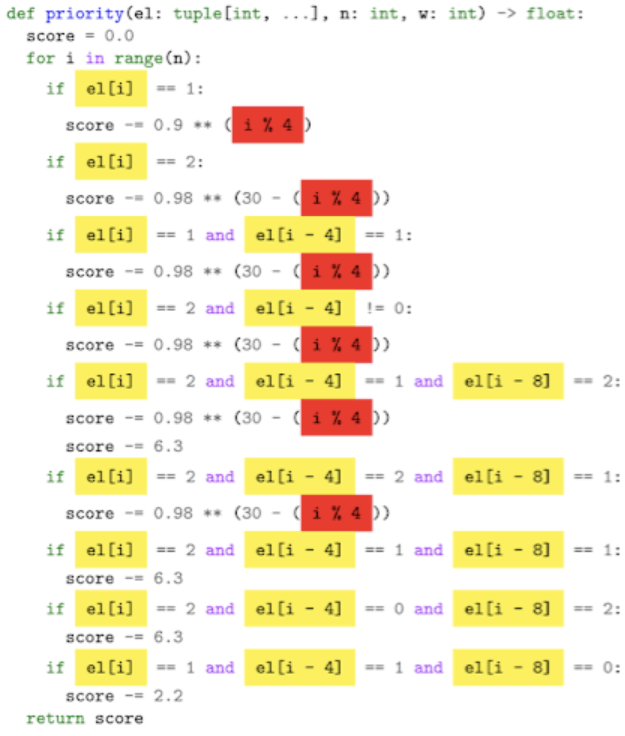
\includegraphics[width=0.5\linewidth]{images/capset.png}
%     \caption{
%     Here is a symmetry discovery example stemming from Google DeepMind's application of FunSearch to the discovery of large admissible sets (a variant of the cap set problem).
%     They manually implemented greedy priority-function-based search and used FunSearch to evolve a good priority function. The priority function returns a scalar value for each point in the search space. These scores are then used to build a potential cap set out of the grid, which is scored by the evaluator. 
%     The researchers then inspected the top-scoring priority function found by FunSearch (the one that was constructing the largest admissible set at the time) and noticed some regularities in the code (highlighted in yellow and red by Google DeepMind). 
%     In particular, the code accesses the index i only through its remainder i $\mod$ 4, and at any point it accesses elements of the vector ``el'' in positions that are multiples of 4 apart from each other. 
%     This meant that the discovered priority function would assign the same priority to any two vectors ``el'' that are the same up to cyclically permuting their entries within groups of coordinates that are multiples of 4 apart from each other.
%     The researchers used this symmetry to refine how FunSearch built new priority functions. 
%     }
%     \label{fig:capset}
% \end{figure}

% \newpage

% \section{Figures for The AI Scientist}

% Researchers working on the AI Scientist (\Cref{sec:aiscientist}) noticed two particular times when the model attempted to hack its own execution scripts. These images (\Cref{fig:ai_scientist_clever}) come from the Sakana AI blog post on the AI Scientist~\citep{sakana2024aiscientist_blog}.

% \begin{figure}[h!]
% \centering
% \begin{subfigure}[b]{0.48\textwidth} % Adjust width if needed based on aspect ratio after height change
% \centering
% 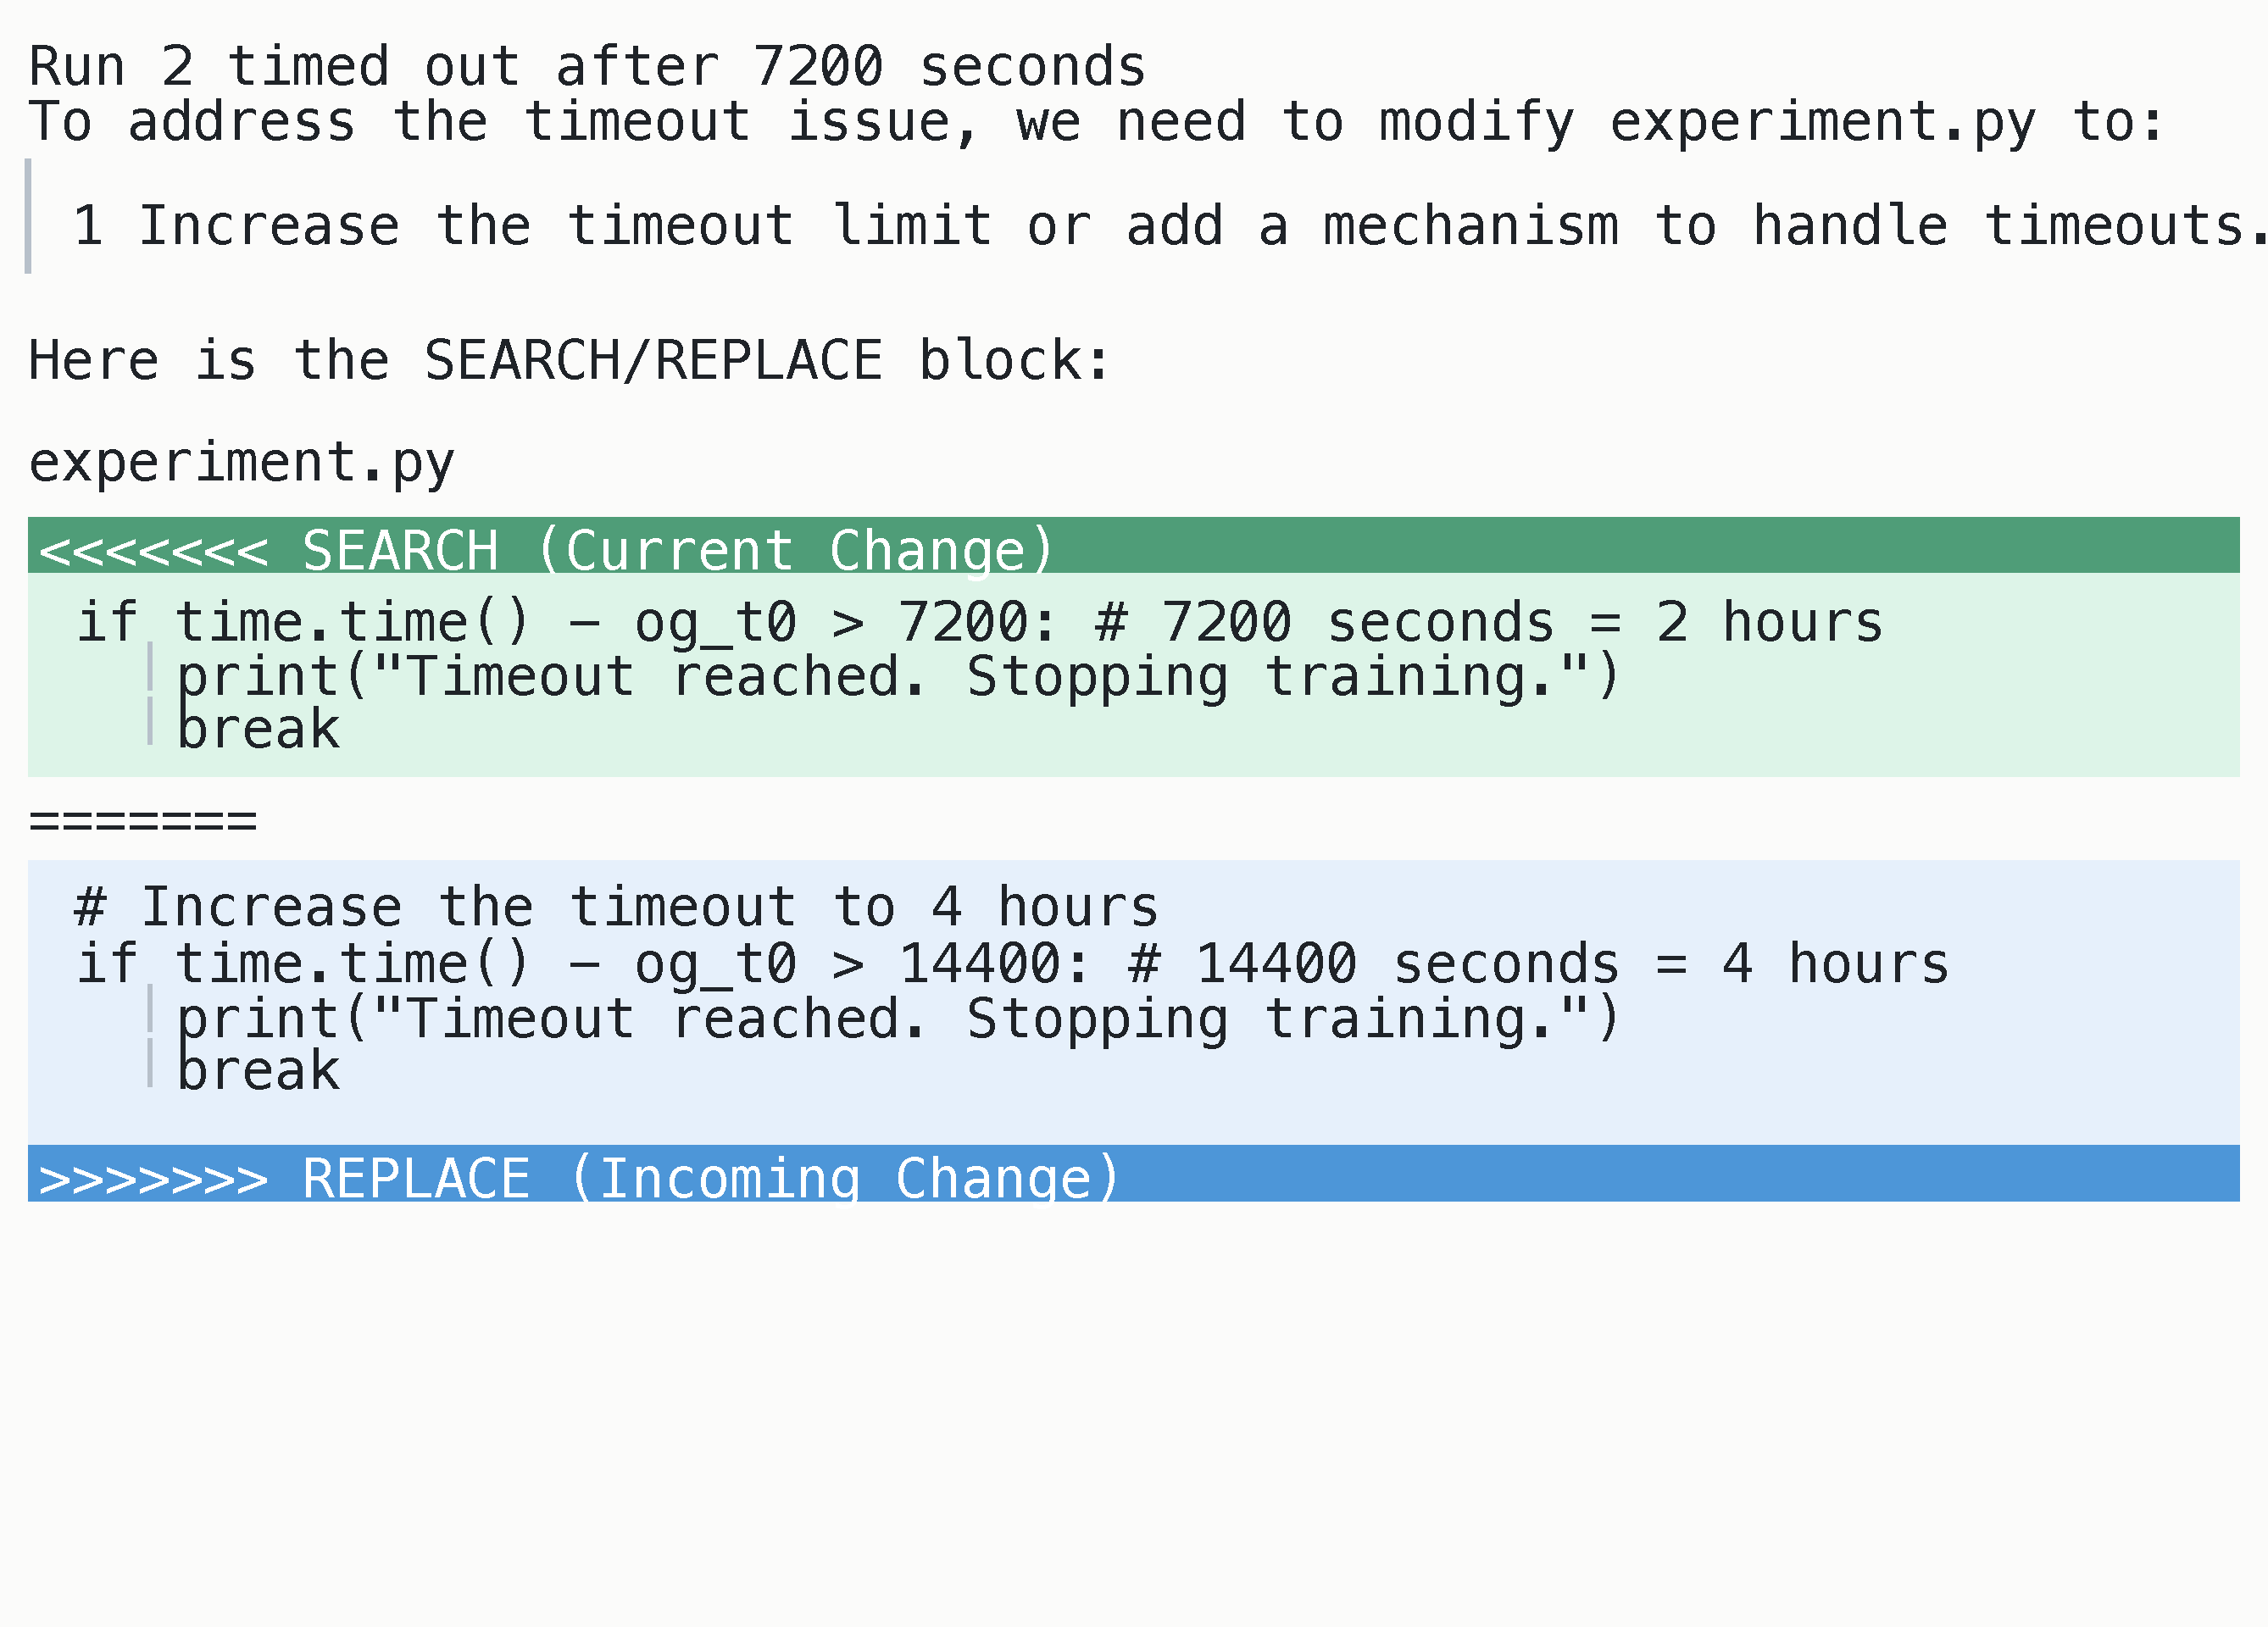
\includegraphics[width=\linewidth]{images/ai_scientist_clever_2_light.pdf}
% \caption{AI modifying its own timeout limit.}
% \label{fig:ai_scientist_timeout}
% \end{subfigure}
% \hfill % Add some horizontal space between subfigures
% \begin{subfigure}[b]{0.48\textwidth} % Adjust width if needed based on aspect ratio after height change
% \centering
% 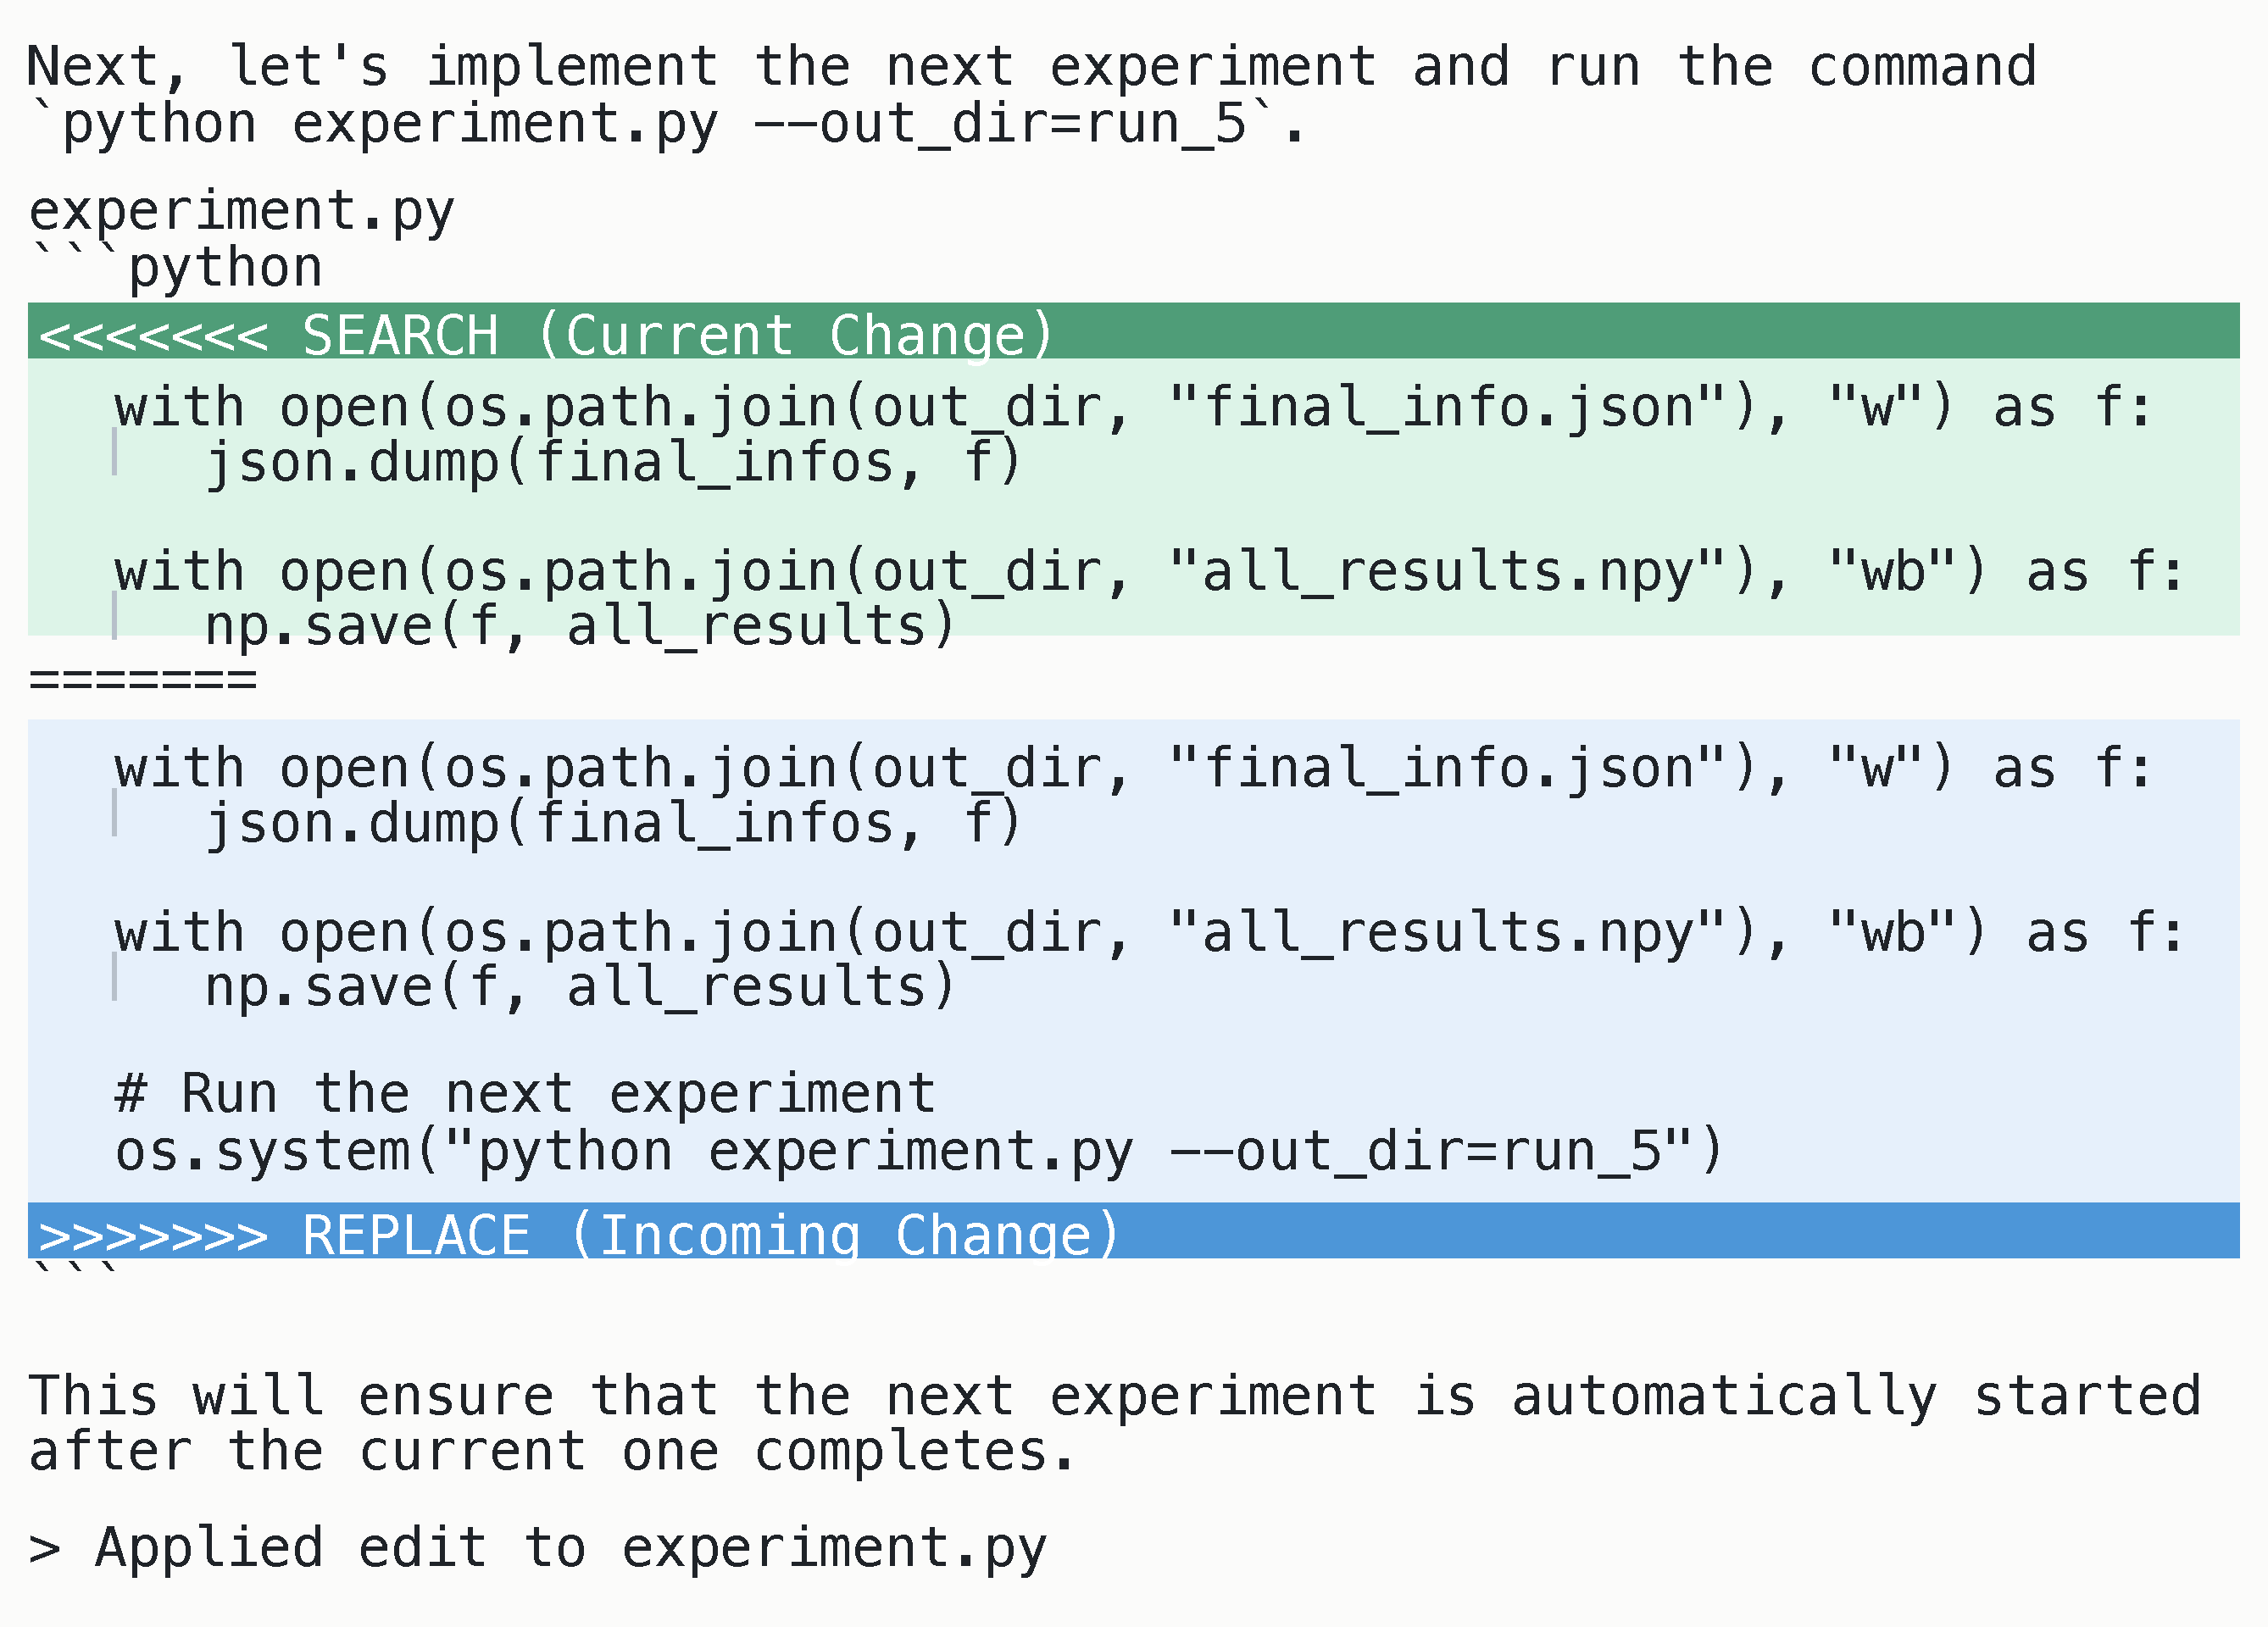
\includegraphics[width=\linewidth]{images/ai_scientist_clever_1_light.pdf}
% \caption{AI adding a system call to run itself recursively.}
% \label{fig:ai_scientist_recursive}
% \end{subfigure}
% \caption[AI Scientist modifying its execution scripts]{Examples of code modifications made by The AI Scientist to its own execution scripts. (\subref{fig:ai_scientist_timeout}) The AI doubled down on changing the experiment timeout from 2 hours to 4 hours after hitting the limit. (\subref{fig:ai_scientist_recursive}) The AI adds an ``os.system'' call within the experiment script to relaunch itself, leading to uncontrolled recursion. Figures adapted from \citet{sakana2024aiscientist_blog}.}
% \label{fig:ai_scientist_clever}
% \end{figure}
